\begin{frame}{Alert Production: Recent achievements}

\begin{itemize}
\item{\texttt{SkyWcs}}
\item{Jointcal: replacing meas\_mosaic}
\item{Alert distribution system: benchmarking \& technology}
\item{End-to-end pipeline, incl. LDM-503-3}
\item{Stack DCR}
\end{itemize}

\end{frame}

\begin{frame}{Data Release Production}

\only<1-2>{
\textbf{LDM-503-2: HSC reprocessing milestone}

\begin{itemize}

  \item{First (equal) post-replan, NSF-visible milestone hit by the project.}
  \item{Joint effort to reprocess (LDF team) and analyze (DRP team) HSC data
  under operations-like conditions}
  \item{Milestone successful!}

\end{itemize}
}

\invisible<1>{
  \textbf{``Warp Compare'' coadds}

  \begin{itemize}
    \item{New algorithm to robustly reject artefacts when coadding images.}
    \item{Now default for HSC processing; stack-wide default to be RFCed soon.}
  \end{itemize}

  \begin{center}
  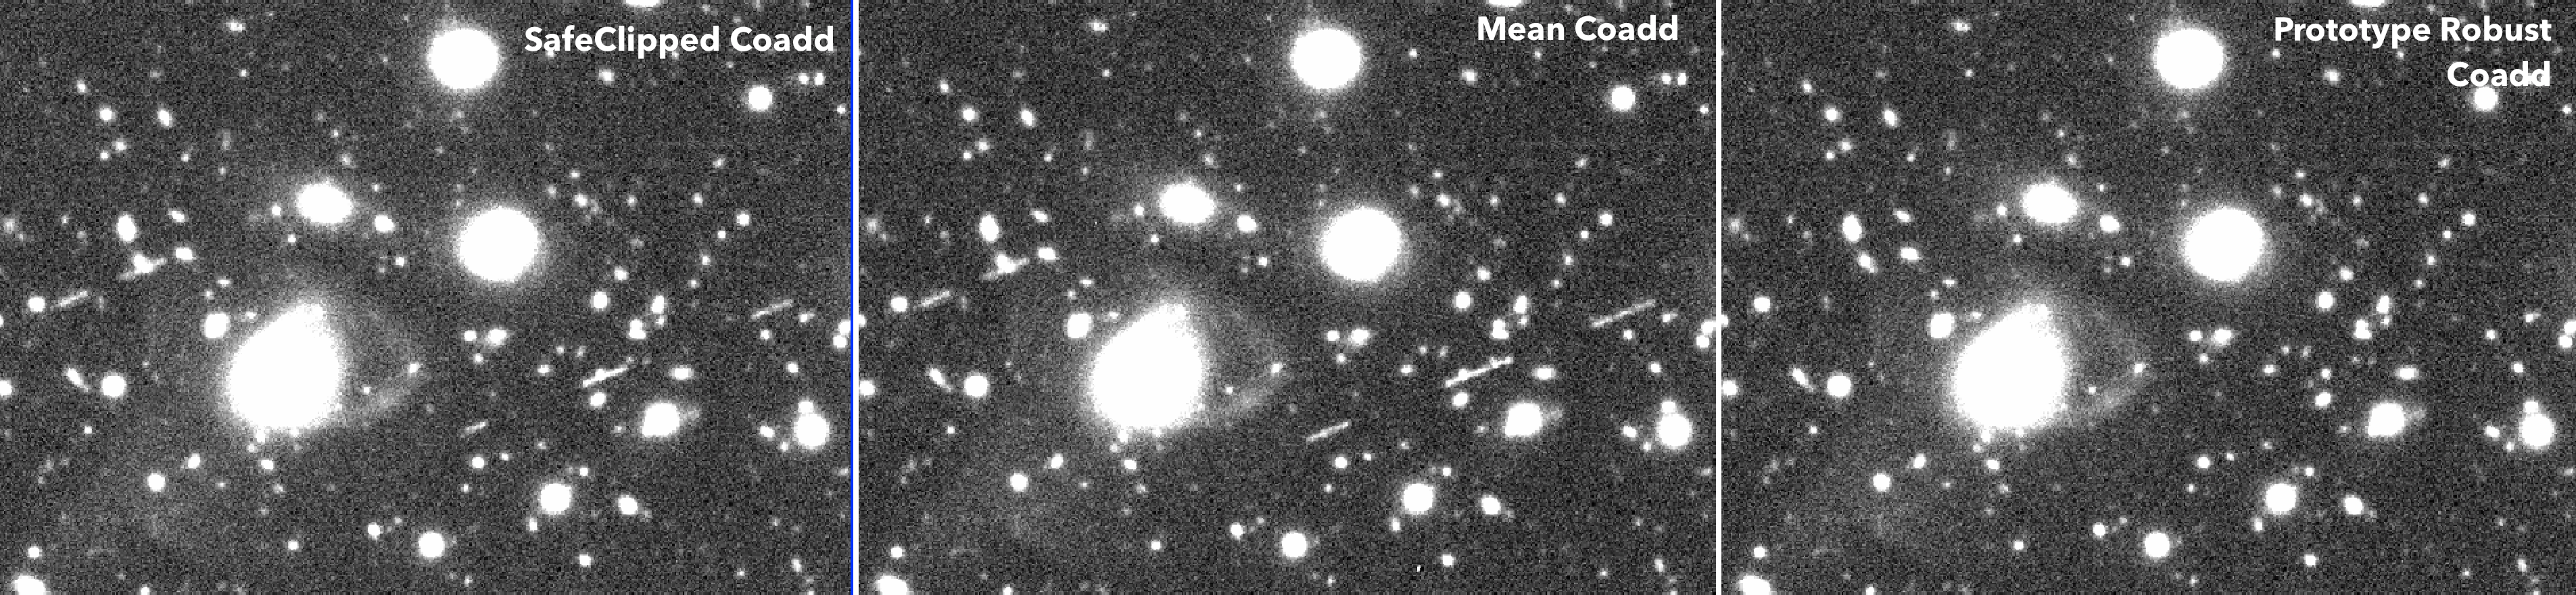
\includegraphics[width=0.5\textwidth]{figures/warpcompare.png}\\
  \tiny Figure: AlSayyad.
  \end{center}
}

\end{frame}

\begin{frame}{Data Release Production}

\textbf{Scarlet: the ``new deblender''}

\begin{itemize}
 \only<1-2>{\item{Key pipeline component; separates overlapping astrophysical objects
 into their constitutent components for measurement.}
  \item{Recent activities:
    \begin{itemize}
      \item{Prototype code developed over the last $\sim$year with exceptionally
      promising results.}
      \item{Journal paper describing the algorithm submitted.}
    \end{itemize}
  }}
  \invisible<1>{\item{Coming up:
    \begin{itemize}
      \item{Performance optimization.}
      \item{Demonstrate performance at-scale on real data with real
      pathologies.}
      \item{Considering how deblender results should affect our approach to
      measurement.}
    \end{itemize}
  }}
\end{itemize}

\begin{center}
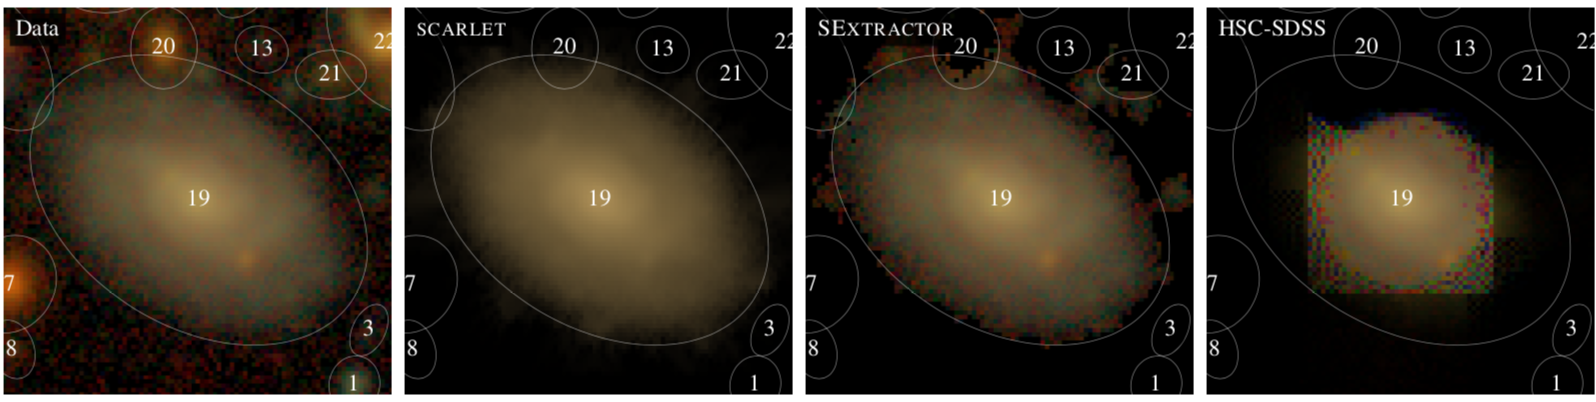
\includegraphics[width=0.5\textwidth]{figures/scarlet.png}\\
\tiny Figure: Melchior et al., 2018
\end{center}

\end{frame}

\begin{frame}{Data Release Production}

\only<1-2>{
  \textbf{``Clever'' coadds}
  \begin{itemize}
    \item{Investigating to what extent we could refine our coaddition techniques
    to enable us to meet our requirements on galaxy shear by measuring
    \textit{only} on coadds (i.e., avoiding the cost \& complexity of MultiFit).}
    \item{Still a work in progress... watch this space.}
  \end{itemize}
}

\invisible<1>{
\textbf{Calibration products \& Auxiliary Telescope}
  \begin{itemize}
    \item{First version of calibration products pipeline added to stack: the
    cp\_pipe package.}
    \item{Currently working on Brighter-Fatter mitigation.}
    \item{Expecting to start on collimated beam projector analysis in F17.}
    \item{Major push on AuxTel spectrophotometric pipeline this year:
    intensive planning in January; tests planned for May \& August; aiming for
    prototype pipeline late summer followed by stack integration.}
  \end{itemize}
}

\end{frame}

\begin{frame}{Data Release Production}

\only<1-2>{
\textbf{``QA'' on HSC data}
\begin{itemize}

  \item{Continued effort to flush out and eliminate all the weird issues that
  crop up when we run the DRP pipelines at scale.}
  \item{Plus: new tooling! Come and learn all about it at the Wednesday
  morning session.}
\end{itemize}
}

\invisible<1>{
\textbf{Do(ough)nuts!}
  \begin{itemize}
    \item{...or rather: using out-of-focus images of stars to measure the
    wavefront, then using that to derive the PSF due to the optical system (as
    opposed to the atmosphere).}
    \item{See results in \citeds{DMTN-064}.}
  \end{itemize}

  \begin{center}
  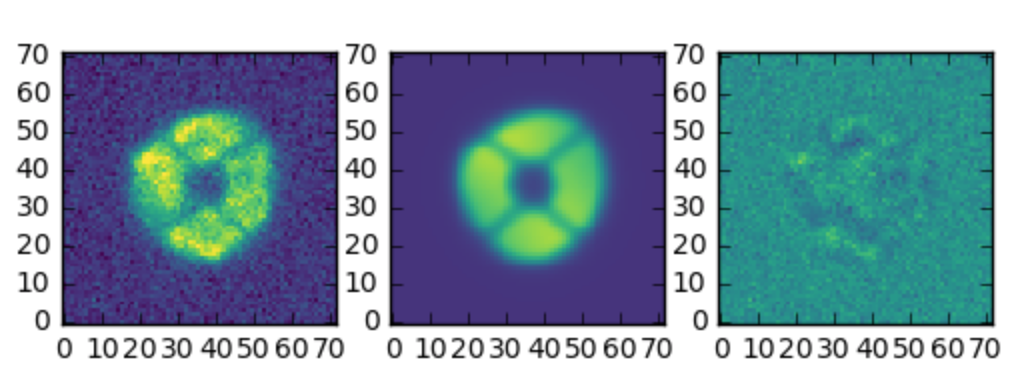
\includegraphics[width=0.5\textwidth]{figures/donut.png}\\
  \tiny Figure: Meyers, \citeds{DMTN-064}
  \end{center}
}

\end{frame}

\begin{frame}{Data Release Production}

\textbf{And more!}
\begin{itemize}

  \item{Work getting started on:

    \begin{itemize}

      \item{Star-galaxy separation}
      \item{New galaxy fitting algorithm}

    \end{itemize}

    ... watch for news at the LSST 2018 Joint Technical Meeting.}

    \item{Lots of effort going into Butler Generation 3.}

\end{itemize}

\end{frame}
